\documentclass{article}
\usepackage{graphicx}
\usepackage[top=.2in,bottom=.2in]{geometry}
\pagestyle{empty}
\usepackage{multicol}
\columnseprule=0.4pt



\begin{document}

\hfill\parbox{3.5in}{\raggedleft Student Name: \rule{2in}{1pt}  }

\bigskip

\bigskip

\bigskip

\begin{centering}
{\Large \sffamily Introduction to Statistical Modeling}\\
\bigskip
%{\Large \sffamily \bfseries Election Eve Projection}\\
%\bigskip
{\Large \sffamily \bfseries{Likelihood and the Election}}\\
\bigskip
\end{centering}

Who is going to win the presidential election?  We don't know yet, but we do have some information that can be encoded in the form of probabilities.

Here is a graphic from Nate Silver's ``FiveThirtyEight'' blog, whose name refers to the number of presidential electoral votes.  The graphic assigns a probability to each possible outcomes over the likely range.  To win, a candidate needs 270 electoral votes.


\bigskip

\centerline{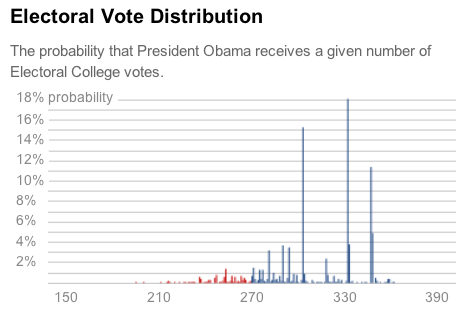
\includegraphics[width=4in]{ElectoralCollege.png}}

\bigskip

Construct your own model of the probability of each possible outcome.  To keep things simple, you should construct your model as a linear combination of four different probability distributions:

\begin{enumerate}

\item Silver's distribution, shown in the graphic.

\item A normal distribution.

\item Another normal distribution.

\item A uniform distribution.

\end{enumerate}

To make your model, specify the parameters and weights for each of the four distributions.  {\bf Your weights must all be non-negative and must add to 1.}

\bigskip

\centerline{\large\begin{tabular}{l|c|cc|cc}
 & & \multicolumn{2}{c}{Params for Normals} & \multicolumn{2}{|c}{Params for Uniform}\\
Distribution & Weight & Mean & Standard Dev. & Min & Max \\\hline\hline
Silver's &  & --- & --- & --- & --- \\\hline
Normal 1 &  &  &  & --- & --- \\\hline
Normal 2 &  &  &  & --- & --- \\\hline
Uniform &  & --- & --- &  &  \\\hline
\end{tabular}}

\bigskip

After the election, we'll evaluate each prediction.  
\begin{quotation}
The prediction with a largest {\bf likelihood} will win \$10.  (Ties to be split.)
\end{quotation}

The ``likelihood,'' a technical term, is the conditional probability p(outcome $|$ model ).  

Of course, both the uniform and normal distribution are continuous.  The electoral vote outcome is discrete.  We'll integrate the model density over the range $\pm 0.5$ around the outcome.

\end{document}